\documentclass[../../main.tex]{subfiles}

%-----------------------------------------------------------%
\begin{document}
\chapter{Instrumentation Sub-system}
\thispagestyle{fancy}

%-----------------------------------------------------------%
% There are two ways to add a section:
%
%
% a) Write the section within the same chapter (Prefer this if the section is small)
%
%
% b) Write a separate section file, and import it to the corresponding chapter (Prefer this if the section is fairly large)
% NOTE: Make sure the names of the (section.tex) are uniquely defined, and easy to read

%\blindtext %remove this command and start writing your own content



%\blindtext %remove this command and start writing your own content

The Instrumentation Sub-system is responsible for capturing star images of required quality for the System. The subsystem is responsible for designing, manufacturing, procuring and testing components like Image sensor, Baffle and Lens in order to meet the requirements 

\section{Image Sensor}
Images sensor is a device which captures photons and gives out digital signal to obtain an image.
The sensor selection is primarily based on the following set of criteria: physical size, power consumption, operating temperature as well as availability. The sensor selection itself is not directly dictated by the star tracker performance requirements but once a sensor is selected, it poses constraints on the lens and the baffle. \par It has been decided that CMOS sensors will be used and not CCDs, mainly due to the extremely low operating temperature of CCDs.
\\We have selected the following sensor according to the constraints
\subsubsection{Python 1300 CMOS Image sensor}
PYTHON 1300 image sensors utilize high sensitivity 4.8 $\mu$ m x 4.8 $\mu$ m pixels with pixel resolution of 1280 x 1024 that support low noise global shutter readout modes, reduced noise and increased dynamic range. The power dissipation is 420mW with operating temperature between -40$^o$ C to +85$^o$ C.



\section{Lens}
Lens is an optical device which converges or diverges light by means of refraction. It will be placed just before the image sensor.

\subsection{Image and Lens Specifications Required}
\label{sec:imagespec}
\begin{itemize}
    \item \textbf{Spot size}: at least \textbf{4 pixels}
\\The lens is required to form a good quality image over the entire sensor, which means minimum aberrations in image over the sensor plane. To achieve sub-pixel accuracy we require to form the image of a star( a point sized object at infinity) over a few pixels, which has been decided to be at least 4. This ensures sub-pixel accuracy with centroiding as well as maximum resolving ability for our system while ensuring the sub-pixel accuracy.
 \item At least \textbf{4 stars} in FOV.\\Hence:
          \begin{itemize}
              \item \textbf{FOV} of at least \textbf{8$^{\circ}\times$10$^{\circ}$}.
              \item \textbf{Focal length} of at most \textbf{35mm}. 
          \end{itemize} 
We require to have at least 4 stars in the FOV of the optical system for the Star Matching algorithm to work. FOV being calculated as :
\begin{equation}
    tan(\theta/2)=\frac{L}{2\times f}
\end{equation}
\begin{align*}
    \theta=& FOV
    \\L=& Sensor\:side\:length
    \\f=& Focal\:length\:of\:lens 
\end{align*}
Clearly this formula doesn't say anything about number of stars in the FOV, the required FOV has to be decided using the star catalogue which has been set to a minimum of 8$^{\circ}$ over the smaller dimension of the sensor which gives a focal length of 35mm. Hence we require a minimum FOV of 8$^{\circ}$ and hence a maximum focal length of 35mm.
    \item \textbf{1 \textless f\#\textless 2}
\\Our imaging system has to work in low-light conditions and hence we require to be able to acquire a good amount of light energy on the sensor. To achieve this we require a large enough aperture.

Considering the amount of energy a limiting magnitude star emits, and the losses incurred in that due to transmission through the lens, efficiency of the sensor, and other factors, and further if we divide that light energy onto at least 4 pixels, we have to deal with very small amount of energy being converted to a pixel value. Also considering the noises present in the sensor, we thus have to acquire quite a large amount of energy from the star.
This is "quite large" because of the focal length that we have to maintain, while maintaining the aperture size. From bench marking as well as our considerations we require a focal length to aperture ratio (f\#) between 1 and 2 which is quite small and difficult to achieve considering all other requirements. As the f\# decreases it becomes more difficult to design a lens which can control the aberrations in limits.
\end{itemize}

\subsection{Lens Systems}
Here we specify the lens systems based on just the number of lenses used in the system as all of the lens systems to be considered are for imaging purpose and to achieve the required image quality.
\subsubsection{Single Lens System}
\graphicspath{}
\begin{figure}[h!]
    \centering
    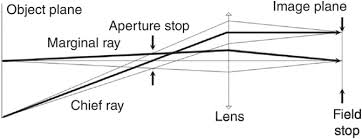
\includegraphics{Figures/Instrumentation/single_lens_system.jpg}
    \caption{Single Lens System showing aperture stop and field stop.}
    \label{fig:8.1}
\end{figure}
\paragraph{Pros:}
\begin{enumerate}
    \item Lower chances of mechanical failure:
    \\Lens being a sensitive object, more the number of lens elements, more the complexity, more the chances of failure  including misalignment of lens elements, breaking, etc. However, certain commercially available star trackers for cubesats have used multiple lens systems.
    \item Low mass:
    \\This depends as we may use a thicker single lens, in place of multiple thinner lenses, but also considering the mass of the lens holder to be used, this can be a factor.
    \item Lowest possible cost:
    \\This factor may also depend on the lens system in consideration, but can be a big differentiator as a single lens generally costs much less than a multi-lens system.
    \item Highest transmission coefficient:
    \\The transmission coefficients ($t$) of general materials for lenses are \textgreater 0.94. The transmission coefficient of a system can be approximated to be $t^n$ where $n$ is the number of lenses used in the system. So a single provides the highest transmission for same aperture diameter. Our system has to work in low light environment so this is a plus point.
\end{enumerate}
\paragraph{Cons:}
\begin{enumerate}
    \item Poor image quality:
    \\For our system we need to minimize only up to the third order optical aberrations namely \textbf{astigmatism, coma, distortion, field curvature }and \textbf{spherical aberration} and also \textbf{chromatic aberrations}. A single lens is not able to reduce all aberrations simultaneously to the required limits over a large enough field (field = FOV). However considering a small FOV we may be able to get the image requirements to be just full filled (More on this in point 3).
    \item Small FOV:
    \\Since a single lens is able to reduce aberrations about the principal axis over a small field, we have to use a small field of view which has to be $\geq8^{\circ}$. Hence the current FOV for a single lens system has been set to $8^{\circ}$.
    \item Limiting spot size:
    \\Achieving a spot size of 4 pixels (i.e. 10$\mu$m diameter) over a field of even $8^{\circ}$ is a challenge for a single lens system while maintaining the range of $f\#$.
    \item f\#:
    \\The required f\# is between 1 and 2 but to maintain the image quality with this f\# for a single lens is a challenge as the spot size increases with decreasing f\#.
    \item Limiting image quality:
    \\The above points in a gist show that the image specifications achieved by a single lens are limiting values and any minor changes in the actual model may lead to a complete change in image, and hence a failure of the system.
\end{enumerate}
\subsubsection{Multiple Lens Systems}
Multiple lens systems not only provide  use of different lenses with different curvatures to get to the required focal length, but also different materials which provides control over chromatic aberrations.

Many refractive optical systems have been devised for imaging. Lens system designing begins with a starting lens system which has been known to work for certain aspects of imaging and then optimising it to suit our needs.



\section{Baffle}
Baffles can be viewed as add-ons to the optical system. They are mainly used to mitigate stray light. It is a conical section, with an entrance window and an exit window which is aligned with the optical axis, that can block the light outside of the FOV.

\subsection{Considerations for Baffle Design}
The parameters and characteristics that must be considered in baffle design are:
\begin{itemize}
    \item \textbf{Dimensions:} Dimensions of the baffle are strongly affected by entrance pupil diameter of optical system, FOV and sun exclusion angle.
    \item \textbf{Vanes arrangement:} Location, size and shape of vanes should be designed to meet the following conditions:
    \begin{itemize}
        \item The vanes should be designed so that none of the optical elements could directly see the places illuminated by intense stray light sources.
        \item The stray light has maximum reflections inside the baffle and between the vanes before reaching the lens.
    \end{itemize}
    \item \textbf{Coating:} The baffle surface must be coated by a black absorbing material.
\end{itemize}

\subsection{Vanes}
Vanes are structures inside the baffle that serve the purpose of blocking all first order stray light from entering the lens. Ideally, baffle and vanes must be designed such that with minimum size and number of vanes, maximum percentage of stray light is attenuated.
\par
\begin{figure}[h]
    \centering
    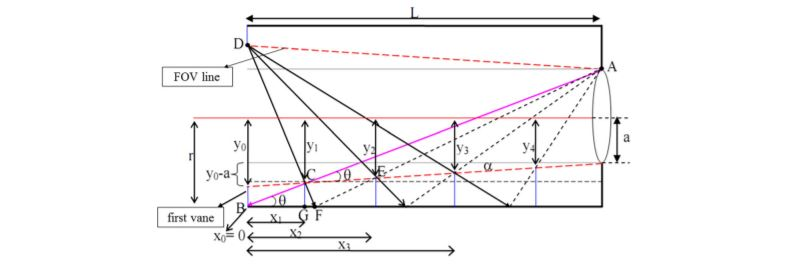
\includegraphics[width=\textwidth]{Figures/Instrumentation/vane_arrangement.JPG}
    \caption{Arrangement of vanes in Baffle by ray tracing}
    \label{fig:8.2}
\end{figure}
The height of the first vane should be determined according to the entrance  aperture diameter, FOV of the system and the baffle length. The position and height of each consequent vane can be determined using the equations:
\begin{center}
    $x_{n+1}=(y_{0}-y_{n+1})\frac{L}{y_{0}-a}$\\
    \vspace{2em}
    $y_{n+1}=r-\frac{r+a}{1+z_{n}} $\\
    \vspace{2em}
    $z_{n}=2a[r-y_{0}+x_{n}\frac{y_{0}-a}{L}\frac{y_{0}+r}{y_{0}+y_{n}}]$
\end{center}
\par
where, $x_{n}$ and $(r-y_{n})$ are the position and height of the $n^{th}$ vane, respectively; $a$ is the semi diameter of the lens; $r$ is the semi diameter of the baffle and $L$ is the length of the baffle.\\

\textbf{\underline{Note:}} The equations mentioned above are obtained by simple ray tracing of stray light.


\subsection{Current Baffle Design}
The following parameters were fixed (based on the Rugged Blue Series M12 imaging lens) before the baffle design was initiated:
\begin{itemize}
    \item \textbf{Aperture of lens system} - 20 $mm$
    \item \textbf{Focal length of lens system} - 12.5 $mm$
    \item \textbf{F number} - 2.5
    \item \textbf{Field of View} - 28.8$^\circ$
\end{itemize}
\par
For determining the length of the baffle, the sun exclusion angle was set to 45$^\circ$ based on data obtained by bench marking and keeping in mind that a higher sun exclusion angle would mean a more effective baffle.
\par
Traditionally, a double baffle is designed for an optical system. The front baffle is a shield against direct sunlight and the rear one attenuates the remaining stray light reflected from the front baffle walls. The single baffle that has been designed is simply the rear baffle. 
%image of baffle here%
\begin{figure}[H]
    \centering
    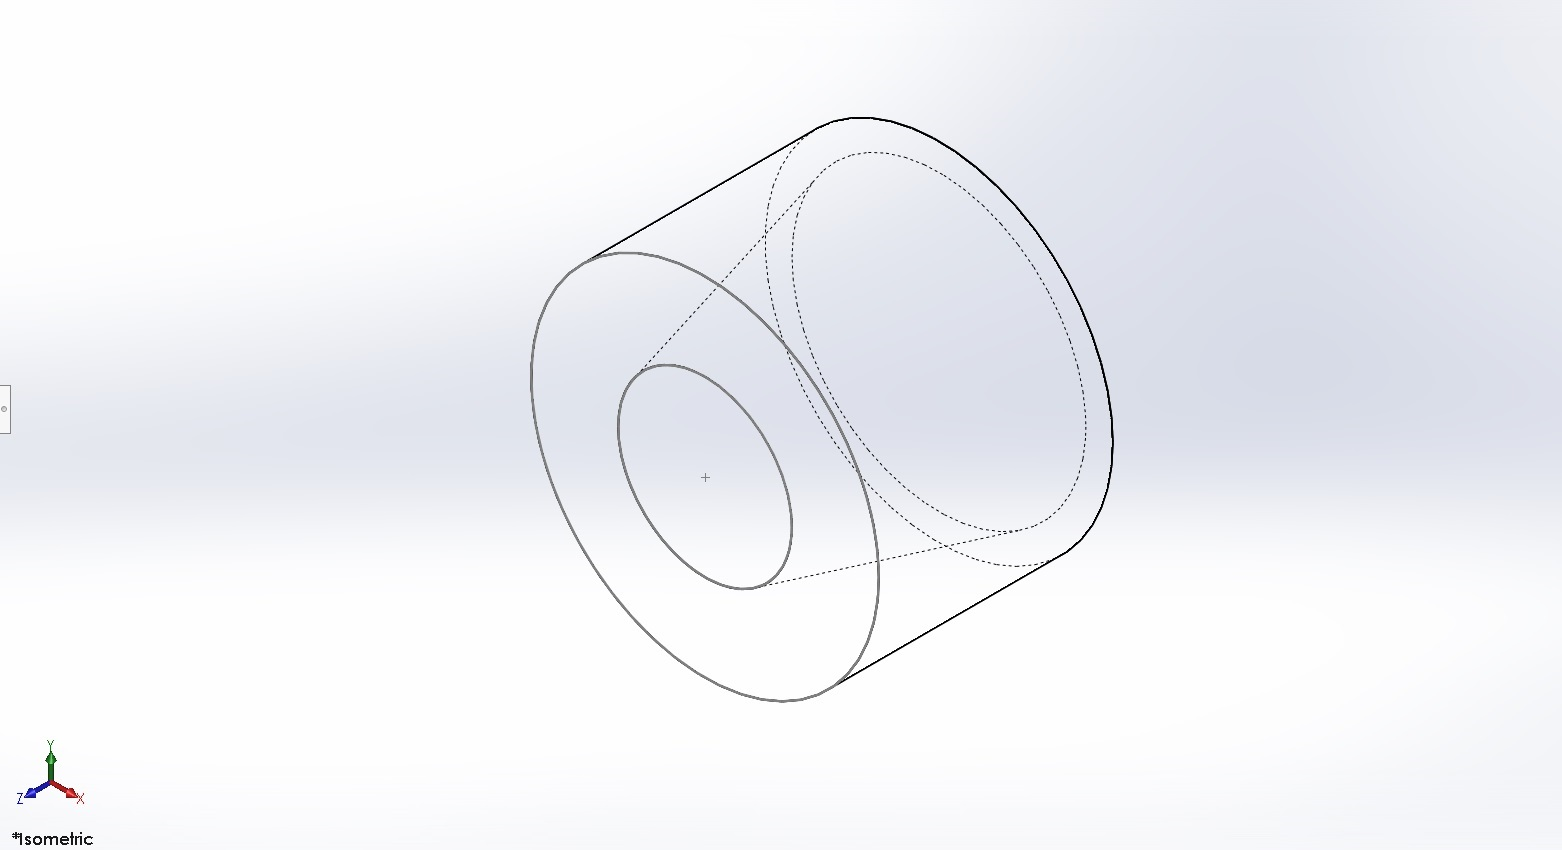
\includegraphics[width=\textwidth]{Figures/Instrumentation/single_baffle.jpg}
    \caption{Isometric view of single baffle without vanes - BAF45003}
    \label{fig:8.3}
\end{figure}

%\section{Interface} Interfacing will be in mech chapter
%this will include all the elements interfacing and how they are placed in order to perform in desired manner
\section{Peripherals}
% we will discus about this
%----------------------------END----------------------------%
\end{document}